\chapter{The Secret Life of Objects}\label{object}

\epigraphhead[30]{
\epigraph{\hspace*{-.1cm}\itshape``An abstract data type is realized by writing a special kind of program […] which defines the type in terms of the operations which can be performed on it.''}%
{---Barbara Liskov, Programming with Abstract Data Types}
}\index{Liskov, Barbara}\index{abstract data type}

\hyperref[data]{Chapter 4} introduced JavaScript's objects. In programming culture, we have a thing called \emph{\index{object-oriented programming}object-oriented programming}, a set of techniques that use objects (and related concepts) as the central principle of program organization.

Though no one really agrees on its precise definition, object-oriented programming has shaped the design of many programming languages, including JavaScript. This chapter will describe the way these ideas can be applied in JavaScript.

\section{Encapsulation}\index{encapsulation}\index{isolation}\index{modularity}

The core idea in object-oriented programming is to divide programs into smaller pieces and make each piece responsible for managing its own state.

This way, some knowledge about the way a piece of the program works can be kept \emph{local} to that piece. Someone working on the rest of the program does not have to remember or even be aware of that knowledge. Whenever these local details change, only the code directly around it needs to be updated.\index{interface!object}

\label{object.interface}Different pieces of such a program interact with each other through \emph{interfaces}, limited sets of functions or bindings that provide useful functionality at a more abstract level, hiding their precise implementation.\index{public properties}\index{private properties}\index{access control}\index{method!interface}

Such program pieces are modeled using \index{object}objects. Their interface consists of a specific set of methods and properties. Properties that are part of the interface are called \emph{public}. The others, which outside code should not be touching, are called \emph{private}.\index{underscore character}

Many languages provide a way to distinguish public and private properties and prevent outside code from accessing the private ones altogether. JavaScript, once again taking the minimalist approach, does not—not yet at least. There is work underway to add this to the language.

Even though the language doesn't have this distinction built in, JavaScript programmers \emph{are} successfully using this idea. Typically, the available interface is described in documentation or comments. It is also common to put an underscore (\lstinline`_`) character at the start of property names to indicate that those properties are private.

Separating interface from implementation is a great idea. It is usually called \emph{\index{encapsulation}encapsulation}.

\label{object.obj_methods}\section{Methods}\index{rabbit example}\index{method}\index{property!access}

Methods are nothing more than properties that hold function values. This is a simple method:

\begin{lstlisting}
let rabbit = {};
rabbit.speak = function(line) {
  console.log(`The rabbit says '${line}'`);
};

rabbit.speak("I'm alive.");
// → The rabbit says 'I'm alive.'
\end{lstlisting}
\noindent\index{this binding}\index{method call}

Usually a method needs to do something with the object it was called on. When a function is called as a method—looked up as a property and immediately called, as in \lstinline`object.method()`—the binding called \lstinline`this` in its body automatically points at the object that it was called on.

\begin{lstlisting}
function speak(line) {
  console.log(`The ${this.type} rabbit says '${line}'`);
}
let whiteRabbit = {type: "white", speak};
let hungryRabbit = {type: "hungry", speak};

whiteRabbit.speak("Oh my ears and whiskers, " +
                  "how late it's getting!");
// → The white rabbit says 'Oh my ears and whiskers, how
//   late it's getting!'
hungryRabbit.speak("I could use a carrot right now.");
// → The hungry rabbit says 'I could use a carrot right now.'
\end{lstlisting}
\noindent\index{call method}

\label{object.call_method}You can think of \lstinline`this` as an extra \index{parameter}parameter that is passed in a different way. If you want to pass it explicitly, you can use a function's \lstinline`call` method, which takes the \lstinline`this` value as its first argument and treats further arguments as normal parameters.

\begin{lstlisting}
speak.call(hungryRabbit, "Burp!");
// → The hungry rabbit says 'Burp!'
\end{lstlisting}
\noindent

Since each function has its own \lstinline`this` binding, whose value depends on the way it is called, you cannot refer to the \lstinline`this` of the wrapping scope in a regular function defined with the \lstinline`function` keyword.\index{this binding}\index{arrow function}

Arrow functions are different—they do not bind their own \lstinline`this` but can see the \lstinline`this` binding of the scope around them. Thus, you can do something like the following code, which references \lstinline`this` from inside a local function:

\begin{lstlisting}
function normalize() {
  console.log(this.coords.map(n => n / this.length));
}
normalize.call({coords: [0, 2, 3], length: 5});
// → [0, 0.4, 0.6]
\end{lstlisting}
\noindent\index{map method}

If I had written the argument to \lstinline`map` using the \lstinline`function` keyword, the code wouldn't work.

\label{object.prototypes}\section{Prototypes}\index{toString method}

Watch closely.

\begin{lstlisting}
let empty = {};
console.log(empty.toString);
// → function toString(){…}
console.log(empty.toString());
// → [object Object]
\end{lstlisting}
\noindent\index{magic}

I pulled a property out of an empty object. Magic!\index{property!inheritance}\index{object!property}

Well, not really. I have simply been withholding information about the way JavaScript objects work. In addition to their set of properties, most objects also have a \emph{\index{prototype}prototype}. A prototype is another object that is used as a fallback source of properties. When an object gets a request for a property that it does not have, its prototype will be searched for the property, then the prototype's prototype, and so on.\index{Object prototype}

So who is the \index{prototype}prototype of that empty object? It is the great ancestral prototype, the entity behind almost all objects, \lstinline`Object.prototype`.

\begin{lstlisting}
console.log(Object.getPrototypeOf({}) ==
            Object.prototype);
// → true
console.log(Object.getPrototypeOf(Object.prototype));
// → null
\end{lstlisting}
\noindent\index{getPrototypeOf function}

As you guess, \lstinline`Object.getPrototypeOf` returns the prototype of an object.\index{toString method}

The prototype relations of JavaScript objects form a \index{tree}tree-shaped structure, and at the root of this structure sits \lstinline`Object.prototype`. It provides a few methods that show up in all objects, such as \lstinline`toString`, which converts an object to a string representation.\index{inheritance}\index{Function prototype}\index{Array prototype}\index{Object prototype}

Many objects don't directly have \lstinline`Object.prototype` as their \index{prototype}prototype but instead have another object that provides a different set of default properties. Functions derive from \lstinline`Function.prototype`, and arrays derive from \lstinline`Array.prototype`.

\begin{lstlisting}
console.log(Object.getPrototypeOf(Math.max) ==
            Function.prototype);
// → true
console.log(Object.getPrototypeOf([]) ==
            Array.prototype);
// → true
\end{lstlisting}
\noindent\index{Object prototype}

Such a prototype object will itself have a prototype, often \lstinline`Object.prototype`, so that it still indirectly provides methods like \lstinline`toString`.\index{rabbit example}\index{Object.create function}

You can use \lstinline`Object.create` to create an object with a specific \index{prototype}prototype.

\begin{lstlisting}
let protoRabbit = {
  speak(line) {
    console.log(`The ${this.type} rabbit says '${line}'`);
  }
};
let killerRabbit = Object.create(protoRabbit);
killerRabbit.type = "killer";
killerRabbit.speak("SKREEEE!");
// → The killer rabbit says 'SKREEEE!'
\end{lstlisting}
\noindent\index{shared property}

A property like \lstinline`speak(line)` in an object expression is a shorthand way of defining a method. It creates a property called \lstinline`speak` and gives it a function as its value.

The ``proto'' rabbit acts as a container for the properties that are shared by all rabbits. An individual rabbit object, like the killer rabbit, contains properties that apply only to itself—in this case its type—and derives shared properties from its prototype.

\label{object.classes}\section{Classes}\index{object-oriented programming}

JavaScript's \index{prototype}prototype system can be interpreted as a somewhat informal take on an object-oriented concept called \emph{\index{class}classes}. A class defines the shape of a type of object—what methods and properties it has. Such an object is called an \emph{\index{instance}instance} of the class.\index{property!inheritance}

Prototypes are useful for defining properties for which all instances of a class share the same value, such as \index{method}methods. Properties that differ per instance, such as our rabbits' \lstinline`type` property, need to be stored directly in the objects themselves.

\label{object.constructors}So to create an instance of a given class, you have to make an object that derives from the proper prototype, but you \emph{also} have to make sure it, itself, has the properties that instances of this class are supposed to have. This is what a \emph{\index{constructor}constructor} function does.

\begin{lstlisting}
function makeRabbit(type) {
  let rabbit = Object.create(protoRabbit);
  rabbit.type = type;
  return rabbit;
}
\end{lstlisting}
\noindent\index{new operator}\index{this binding}\index{return keyword}\index{object!creation}

JavaScript provides a way to make defining this type of function easier. If you put the keyword \lstinline`new` in front of a function call, the function is treated as a constructor. This means that an object with the right prototype is automatically created, bound to \lstinline`this` in the function, and returned at the end of the function.\index{prototype property}

The prototype object used when constructing objects is found by taking the \lstinline`prototype` property of the constructor function.\index{rabbit example}

\begin{lstlisting}
function Rabbit(type) {
  this.type = type;
}
Rabbit.prototype.speak = function(line) {
  console.log(`The ${this.type} rabbit says '${line}'`);
};

let weirdRabbit = new Rabbit("weird");
\end{lstlisting}
\noindent\index{constructor}

Constructors (all functions, in fact) automatically get a property named \lstinline`prototype`, which by default holds a plain, empty object that derives from \lstinline`Object.prototype`. You can overwrite it with a new object if you want. Or you can add properties to the existing object, as the example does.\index{capitalization}

By convention, the names of constructors are capitalized so that they can easily be distinguished from other functions.\index{prototype property}\index{getPrototypeOf function}

It is important to understand the distinction between the way a prototype is associated with a constructor (through its \lstinline`prototype` property) and the way objects \emph{have} a prototype (which can be found with \lstinline`Object.getPrototypeOf`). The actual prototype of a constructor is \lstinline`Function.prototype` since constructors are functions. Its \lstinline`prototype` \emph{property} holds the prototype used for instances created through it.

\begin{lstlisting}
console.log(Object.getPrototypeOf(Rabbit) ==
            Function.prototype);
// → true
console.log(Object.getPrototypeOf(weirdRabbit) ==
            Rabbit.prototype);
// → true
\end{lstlisting}
\noindent

\section{Class notation}

So JavaScript \index{class}classes are \index{constructor}constructor functions with a \index{prototype}prototype property. That is how they work, and until 2015, that was how you had to write them. These days, we have a less awkward notation.

\begin{lstlisting}
class Rabbit {
  constructor(type) {
    this.type = type;
  }
  speak(line) {
    console.log(`The ${this.type} rabbit says '${line}'`);
  }
}

let killerRabbit = new Rabbit("killer");
let blackRabbit = new Rabbit("black");
\end{lstlisting}
\noindent\index{rabbit example}\index{braces!class}

The \lstinline`class` keyword starts a \index{class declaration}class declaration, which allows us to define a constructor and a set of methods all in a single place. Any number of methods may be written inside the declaration's braces. The one named \lstinline`constructor` is treated specially. It provides the actual constructor function, which will be bound to the name \lstinline`Rabbit`. The others are packaged into that constructor's prototype. Thus, the earlier class declaration is equivalent to the constructor definition from the previous section. It just looks nicer.\index{class declaration!properties}

Class declarations currently allow only \emph{methods}—properties that hold functions—to be added to the \index{prototype}prototype. This can be somewhat inconvenient when you want to save a non-function value in there. The next version of the language will probably improve this. For now, you can create such properties by directly manipulating the prototype after you've defined the class.

Like \lstinline`function`, \lstinline`class` can be used both in statements and in expressions. When used as an expression, it doesn't define a binding but just produces the constructor as a value. You are allowed to omit the class name in a class expression.

\begin{lstlisting}
let object = new class { getWord() { return "hello"; } };
console.log(object.getWord());
// → hello
\end{lstlisting}
\noindent

\section{Overriding derived properties}\index{shared property}\index{overriding}\index{property!inheritance}

When you add a property to an object, whether it is present in the prototype or not, the property is added to the object \emph{itself}. If there was already a property with the same name in the prototype, this property will no longer affect the object, as it is now hidden behind the object's own property.

\begin{lstlisting}
Rabbit.prototype.teeth = "small";
console.log(killerRabbit.teeth);
// → small
killerRabbit.teeth = "long, sharp, and bloody";
console.log(killerRabbit.teeth);
// → long, sharp, and bloody
console.log(blackRabbit.teeth);
// → small
console.log(Rabbit.prototype.teeth);
// → small
\end{lstlisting}
\noindent\index{prototype!diagram}

The following diagram sketches the situation after this code has run. The \lstinline`Rabbit` and \lstinline`Object` \index{prototype}prototypes lie behind \lstinline`killerRabbit` as a kind of backdrop, where properties that are not found in the object itself can be looked up.

\vskip 1.5ex
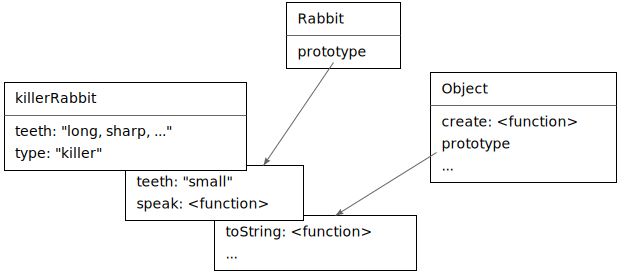
\includegraphics[width=8cm]{img/generated/rabbits.pdf}
\vskip 1.5ex\index{shared property}

Overriding properties that exist in a prototype can be a useful thing to do. As the rabbit teeth example shows, overriding can be used to express exceptional properties in instances of a more generic class of objects, while letting the nonexceptional objects take a standard value from their prototype.\index{toString method}\index{Array prototype}\index{Function prototype}

Overriding is also used to give the standard function and array prototypes a different \lstinline`toString` method than the basic object prototype.

\begin{lstlisting}
console.log(Array.prototype.toString ==
            Object.prototype.toString);
// → false
console.log([1, 2].toString());
// → 1,2
\end{lstlisting}
\noindent\index{toString method}\index{join method}\index{call method}

Calling \lstinline`toString` on an array gives a result similar to calling \lstinline`.join(",")` on it—it puts commas between the values in the array. Directly calling \lstinline`Object.prototype.toString` with an array produces a different string. That function doesn't know about arrays, so it simply puts the word \emph{object} and the name of the type between square brackets.

\begin{lstlisting}
console.log(Object.prototype.toString.call([1, 2]));
// → [object Array]
\end{lstlisting}
\noindent

\section{Maps}\index{map method}

We saw the word \emph{map} used in the \hyperref[higher_order.map]{previous chapter} for an operation that transforms a data structure by applying a function to its elements. Confusing as it is, in programming the same word is also used for a related but rather different thing.\index{map (data structure)}\index{ages example}\index{data structure!map}

A \emph{map} (noun) is a data structure that associates values (the keys) with other values. For example, you might want to map names to ages. It is possible to use objects for this.

\begin{lstlisting}
let ages = {
  Boris: 39,
  Liang: 22,
  Júlia: 62
};

console.log(`Júlia is ${ages["Júlia"]}`);
// → Júlia is 62
console.log("Is Jack's age known?", "Jack" in ages);
// → Is Jack's age known? false
console.log("Is toString's age known?", "toString" in ages);
// → Is toString's age known? true
\end{lstlisting}
\noindent\index{Object.prototype}\index{toString method}

Here, the object's property names are the people's names, and the property values are their ages. But we certainly didn't list anybody named toString in our map. Yet, because plain objects derive from \lstinline`Object.prototype`, it looks like the property is there.\index{Object.create function}\index{prototype}

As such, using plain objects as maps is dangerous. There are several possible ways to avoid this problem. First, it is possible to create objects with \emph{no} prototype. If you pass \lstinline`null` to \lstinline`Object.create`, the resulting object will not derive from \lstinline`Object.prototype` and can safely be used as a map.

\begin{lstlisting}
console.log("toString" in Object.create(null));
// → false
\end{lstlisting}
\noindent\index{property!naming}

Object property names must be strings. If you need a map whose keys can't easily be converted to strings—such as objects—you cannot use an object as your map.\index{Map class}

Fortunately, JavaScript comes with a class called \lstinline`Map` that is written for this exact purpose. It stores a mapping and allows any type of keys.

\begin{lstlisting}
let ages = new Map();
ages.set("Boris", 39);
ages.set("Liang", 22);
ages.set("Júlia", 62);

console.log(`Júlia is ${ages.get("Júlia")}`);
// → Júlia is 62
console.log("Is Jack's age known?", ages.has("Jack"));
// → Is Jack's age known? false
console.log(ages.has("toString"));
// → false
\end{lstlisting}
\noindent\index{interface!object}\index{set method}\index{get method}\index{has method}\index{encapsulation}

The methods \lstinline`set`, \lstinline`get`, and \lstinline`has` are part of the interface of the \lstinline`Map` object. Writing a data structure that can quickly update and search a large set of values isn't easy, but we don't have to worry about that. Someone else did it for us, and we can go through this simple interface to use their work.\index{hasOwnProperty method}\index{in operator}

If you do have a plain object that you need to treat as a map for some reason, it is useful to know that \lstinline`Object.keys` returns only an object's \emph{own} keys, not those in the prototype. As an alternative to the \lstinline`in` operator, you can use the \lstinline`hasOwnProperty` method, which ignores the object's prototype.

\begin{lstlisting}
console.log({x: 1}.hasOwnProperty("x"));
// → true
console.log({x: 1}.hasOwnProperty("toString"));
// → false
\end{lstlisting}
\noindent

\section{Polymorphism}\index{toString method}\index{String function}\index{polymorphism}\index{overriding}\index{object-oriented programming}

When you call the \lstinline`String` function (which converts a value to a string) on an object, it will call the \lstinline`toString` method on that object to try to create a meaningful string from it. I mentioned that some of the standard prototypes define their own version of \lstinline`toString` so they can create a string that contains more useful information than \lstinline`"[object Object]"`. You can also do that yourself.

\begin{lstlisting}
Rabbit.prototype.toString = function() {
  return `a ${this.type} rabbit`;
};

console.log(String(blackRabbit));
// → a black rabbit
\end{lstlisting}
\noindent\index{object-oriented programming}\index{interface!object}

This is a simple instance of a powerful idea. When a piece of code is written to work with objects that have a certain interface—in this case, a \lstinline`toString` method—any kind of object that happens to support this interface can be plugged into the code, and it will just work.

This technique is called \emph{polymorphism}. Polymorphic code can work with values of different shapes, as long as they support the interface it expects.\index{for/of loop}\index{iterator interface}

I mentioned in \hyperref[data.for_of_loop]{Chapter 4} that a \lstinline`for`/\lstinline`of` loop can loop over several kinds of data structures. This is another case of polymorphism—such loops expect the data structure to expose a specific interface, which arrays and strings do. And we can also add this interface to your own objects! But before we can do that, we need to know what symbols are.

\section{Symbols}

It is possible for multiple interfaces to use the same property name for different things. For example, I could define an interface in which the \lstinline`toString` method is supposed to convert the object into a piece of yarn. It would not be possible for an object to conform to both that interface and the standard use of \lstinline`toString`.

That would be a bad idea, and this problem isn't that common. Most JavaScript programmers simply don't think about it. But the language designers, whose \emph{job} it is to think about this stuff, have provided us with a solution anyway.\index{Symbol function}\index{property!naming}

When I claimed that property names are strings, that wasn't entirely accurate. They usually are, but they can also be \emph{\index{symbol}symbols}. Symbols are values created with the \lstinline`Symbol` function. Unlike strings, newly created symbols are unique—you cannot create the same symbol twice.

\begin{lstlisting}
let sym = Symbol("name");
console.log(sym == Symbol("name"));
// → false
Rabbit.prototype[sym] = 55;
console.log(blackRabbit[sym]);
// → 55
\end{lstlisting}
\noindent

The string you pass to \lstinline`Symbol` is included when you convert it to a string and can make it easier to recognize a symbol when, for example, showing it in the console. But it has no meaning beyond that—multiple symbols may have the same name.

Being both unique and usable as property names makes symbols suitable for defining interfaces that can peacefully live alongside other properties, no matter what their names are.

\begin{lstlisting}
const toStringSymbol = Symbol("toString");
Array.prototype[toStringSymbol] = function() {
  return `${this.length} cm of blue yarn`;
};

console.log([1, 2].toString());
// → 1,2
console.log([1, 2][toStringSymbol]());
// → 2 cm of blue yarn
\end{lstlisting}
\noindent\index{property!naming}

It is possible to include symbol properties in object expressions and classes by using \index{square bracket}square brackets around the property name. That causes the property name to be evaluated, much like the square bracket property access notation, which allows us to refer to a binding that holds the symbol.

\begin{lstlisting}
let stringObject = {
  [toStringSymbol]() { return "a jute rope"; }
};
console.log(stringObject[toStringSymbol]());
// → a jute rope
\end{lstlisting}
\noindent

\section{The iterator interface}\index{iterable interface}\index{Symbol.iterator symbol}\index{for/of loop}

The object given to a \lstinline`for`/\lstinline`of` loop is expected to be \emph{iterable}. This means it has a method named with the \lstinline`Symbol.iterator` symbol (a symbol value defined by the language, stored as a property of the \lstinline`Symbol` function).\index{iterator interface}\index{next method}

When called, that method should return an object that provides a second interface, \emph{iterator}. This is the actual thing that iterates. It has a \lstinline`next` method that returns the next result. That result should be an object with a \lstinline`value` property that provides the next value, if there is one, and a \lstinline`done` property, which should be true when there are no more results and false otherwise.

Note that the \lstinline`next`, \lstinline`value`, and \lstinline`done` property names are plain strings, not symbols. Only \lstinline`Symbol.iterator`, which is likely to be added to a \emph{lot} of different objects, is an actual symbol.

We can directly use this interface ourselves.

\begin{lstlisting}
let okIterator = "OK"[Symbol.iterator]();
console.log(okIterator.next());
// → {value: "O", done: false}
console.log(okIterator.next());
// → {value: "K", done: false}
console.log(okIterator.next());
// → {value: undefined, done: true}
\end{lstlisting}
\noindent\index{matrix example}\index{Matrix class}\index{array!as matrix}

\label{object.matrix}Let's implement an iterable data structure. We'll build a \emph{matrix} class, acting as a two-dimensional array.

\begin{lstlisting}
class Matrix {
  constructor(width, height, element = (x, y) => undefined) {
    this.width = width;
    this.height = height;
    this.content = [];

    for (let y = 0; y < height; y++) {
      for (let x = 0; x < width; x++) {
        this.content[y * width + x] = element(x, y);
      }
    }
  }

  get(x, y) {
    return this.content[y * this.width + x];
  }
  set(x, y, value) {
    this.content[y * this.width + x] = value;
  }
}
\end{lstlisting}
\noindent

The class stores its content in a single array of \emph{width} × \emph{height} elements. The elements are stored row by row, so, for example, the third element in the fifth row is (using zero-based indexing) stored at position 4 × \emph{width} + 2.

The constructor function takes a width, a height, and an optional \lstinline`element` function that will be used to fill in the initial values. There are \lstinline`get` and \lstinline`set` methods to retrieve and update elements in the matrix.

When looping over a matrix, you are usually interested in the position of the elements as well as the elements themselves, so we'll have our iterator produce objects with \lstinline`x`, \lstinline`y`, and \lstinline`value` properties.\index{MatrixIterator class}

\begin{lstlisting}
class MatrixIterator {
  constructor(matrix) {
    this.x = 0;
    this.y = 0;
    this.matrix = matrix;
  }

  next() {
    if (this.y == this.matrix.height) return {done: true};

    let value = {x: this.x,
                 y: this.y,
                 value: this.matrix.get(this.x, this.y)};
    this.x++;
    if (this.x == this.matrix.width) {
      this.x = 0;
      this.y++;
    }
    return {value, done: false};
  }
}
\end{lstlisting}
\noindent

The class tracks the progress of iterating over a matrix in its \lstinline`x` and \lstinline`y` properties. The \lstinline`next` method starts by checking whether the bottom of the matrix has been reached. If it hasn't, it \emph{first} creates the object holding the current value and \emph{then} updates its position, moving to the next row if necessary.

Let's set up the \lstinline`Matrix` class to be iterable. Throughout this book, I'll occasionally use after-the-fact prototype manipulation to add methods to classes so that the individual pieces of code remain small and self-contained. In a regular program, where there is no need to split the code into small pieces, you'd declare these methods directly in the class instead.

\begin{lstlisting}
Matrix.prototype[Symbol.iterator] = function() {
  return new MatrixIterator(this);
};
\end{lstlisting}
\noindent\index{for/of loop}

We can now loop over a matrix with \lstinline`for`/\lstinline`of`.

\begin{lstlisting}
let matrix = new Matrix(2, 2, (x, y) => `value ${x},${y}`);
for (let {x, y, value} of matrix) {
  console.log(x, y, value);
}
// → 0 0 value 0,0
// → 1 0 value 1,0
// → 0 1 value 0,1
// → 1 1 value 1,1
\end{lstlisting}
\noindent

\section{Getters, setters, and statics}\index{interface!object}\index{property!definition}\index{Map class}

Interfaces often consist mostly of methods, but it is also okay to include properties that hold non-function values. For example, \lstinline`Map` objects have a \lstinline`size` property that tells you how many keys are stored in them.

It is not even necessary for such an object to compute and store such a property directly in the instance. Even properties that are accessed directly may hide a method call. Such methods are called \emph{\index{getter}getters}, and they are defined by writing \lstinline`get` in front of the method name in an object expression or class declaration.

\begin{lstlisting}
let varyingSize = {
  get size() {
    return Math.floor(Math.random() * 100);
  }
};

console.log(varyingSize.size);
// → 73
console.log(varyingSize.size);
// → 49
\end{lstlisting}
\noindent\index{temperature example}

Whenever someone reads from this object's \lstinline`size` property, the associated method is called. You can do a similar thing when a property is written to, using a \emph{\index{setter}setter}.

\begin{lstlisting}
class Temperature {
  constructor(celsius) {
    this.celsius = celsius;
  }
  get fahrenheit() {
    return this.celsius * 1.8 + 32;
  }
  set fahrenheit(value) {
    this.celsius = (value - 32) / 1.8;
  }

  static fromFahrenheit(value) {
    return new Temperature((value - 32) / 1.8);
  }
}

let temp = new Temperature(22);
console.log(temp.fahrenheit);
// → 71.6
temp.fahrenheit = 86;
console.log(temp.celsius);
// → 30
\end{lstlisting}
\noindent

The \lstinline`Temperature` class allows you to read and write the temperature in either degrees \index{Celsius}Celsius or degrees \index{Fahrenheit}Fahrenheit, but internally it stores only Celsius and automatically converts to and from Celsius in the \lstinline`fahrenheit` getter and setter.\index{static method}

Sometimes you want to attach some properties directly to your constructor function, rather than to the prototype. Such methods won't have access to a class instance but can, for example, be used to provide additional ways to create instances.

Inside a class declaration, methods that have \lstinline`static` written before their name are stored on the constructor. So the \lstinline`Temperature` class allows you to write \lstinline`Temperature.fromFahrenheit(100)` to create a temperature using degrees Fahrenheit.

\section{Inheritance}\index{inheritance}\index{matrix example}\index{object-oriented programming}\index{SymmetricMatrix class}

Some matrices are known to be \emph{symmetric}. If you mirror a symmetric matrix around its top-left-to-bottom-right diagonal, it stays the same. In other words, the value stored at \emph{x},\emph{y} is always the same as that at \emph{y},\emph{x}.

Imagine we need a data structure like \lstinline`Matrix` but one that enforces the fact that the matrix is and remains symmetrical. We could write it from scratch, but that would involve repeating some code very similar to what we already wrote.\index{overriding}\index{prototype}

JavaScript's prototype system makes it possible to create a \emph{new} class, much like the old class, but with new definitions for some of its properties. The prototype for the new class derives from the old prototype but adds a new definition for, say, the \lstinline`set` method.

In object-oriented programming terms, this is called \emph{\index{inheritance}inheritance}. The new class inherits properties and behavior from the old class.

\begin{lstlisting}
class SymmetricMatrix extends Matrix {
  constructor(size, element = (x, y) => undefined) {
    super(size, size, (x, y) => {
      if (x < y) return element(y, x);
      else return element(x, y);
    });
  }

  set(x, y, value) {
    super.set(x, y, value);
    if (x != y) {
      super.set(y, x, value);
    }
  }
}

let matrix = new SymmetricMatrix(5, (x, y) => `${x},${y}`);
console.log(matrix.get(2, 3));
// → 3,2
\end{lstlisting}
\noindent

The use of the word \lstinline`extends` indicates that this class shouldn't be directly based on the default \lstinline`Object` prototype but on some other class. This is called the \emph{\index{superclass}superclass}. The derived class is the \emph{\index{subclass}subclass}.

To initialize a \lstinline`SymmetricMatrix` instance, the constructor calls its superclass's constructor through the \lstinline`super` keyword. This is necessary because if this new object is to behave (roughly) like a \lstinline`Matrix`, it is going to need the instance properties that matrices have. To ensure the matrix is symmetrical, the constructor wraps the \lstinline`element` function to swap the coordinates for values below the diagonal.

The \lstinline`set` method again uses \lstinline`super` but this time not to call the constructor but to call a specific method from the superclass's set of methods. We are redefining \lstinline`set` but do want to use the original behavior. Because \lstinline`this.set` refers to the \emph{new} \lstinline`set` method, calling that wouldn't work. Inside class methods, \lstinline`super` provides a way to call methods as they were defined in the superclass.

Inheritance allows us to build slightly different data types from existing data types with relatively little work. It is a fundamental part of the object-oriented tradition, alongside encapsulation and polymorphism. But while the latter two are now generally regarded as wonderful ideas, inheritance is more controversial.\index{complexity}\index{reuse}\index{class hierarchy}

Whereas \index{encapsulation}encapsulation and polymorphism can be used to \emph{separate} pieces of code from each other, reducing the tangledness of the overall program, \index{inheritance}inheritance fundamentally ties classes together, creating \emph{more} tangle. When inheriting from a class, you usually have to know more about how it works than when simply using it. Inheritance can be a useful tool, and I use it now and then in my own programs, but it shouldn't be the first tool you reach for, and you probably shouldn't actively go looking for opportunities to construct class hierarchies (family trees of classes).

\section{The instanceof operator}\index{type}\index{instanceof operator}\index{constructor}\index{object}

It is occasionally useful to know whether an object was derived from a specific class. For this, JavaScript provides a binary operator called \lstinline`instanceof`.

\begin{lstlisting}
console.log(
  new SymmetricMatrix(2) instanceof SymmetricMatrix);
// → true
console.log(new SymmetricMatrix(2) instanceof Matrix);
// → true
console.log(new Matrix(2, 2) instanceof SymmetricMatrix);
// → false
console.log([1] instanceof Array);
// → true
\end{lstlisting}
\noindent\index{inheritance}

The operator will see through inherited types, so a \lstinline`SymmetricMatrix` is an instance of \lstinline`Matrix`. The operator can also be applied to standard constructors like \lstinline`Array`. Almost every object is an instance of \lstinline`Object`.

\section{Summary}

So objects do more than just hold their own properties. They have prototypes, which are other objects. They'll act as if they have properties they don't have as long as their prototype has that property. Simple objects have \lstinline`Object.prototype` as their prototype.

Constructors, which are functions whose names usually start with a capital letter, can be used with the \lstinline`new` operator to create new objects. The new object's prototype will be the object found in the \lstinline`prototype` property of the constructor. You can make good use of this by putting the properties that all values of a given type share into their prototype. There's a \lstinline`class` notation that provides a clear way to define a constructor and its prototype.

You can define getters and setters to secretly call methods every time an object's property is accessed. Static methods are methods stored in a class's constructor, rather than its prototype.

The \lstinline`instanceof` operator can, given an object and a constructor, tell you whether that object is an instance of that constructor.

One useful thing to do with objects is to specify an interface for them and tell everybody that they are supposed to talk to your object only through that interface. The rest of the details that make up your object are now \emph{encapsulated}, hidden behind the interface.

More than one type may implement the same interface. Code written to use an interface automatically knows how to work with any number of different objects that provide the interface. This is called \emph{polymorphism}.

When implementing multiple classes that differ in only some details, it can be helpful to write the new classes as \emph{subclasses} of an existing class, \emph{inheriting} part of its behavior.

\section{Exercises}

\label{object.exercise_vector}\subsection{A vector type}\index{dimensions}\index{Vec class}\index{coordinates}\index{vector (exercise)}

Write a \index{class}class \lstinline`Vec` that represents a vector in two-dimensional space. It takes \lstinline`x` and \lstinline`y` parameters (numbers), which it should save to properties of the same name.\index{addition}\index{subtraction}

Give the \lstinline`Vec` prototype two methods, \lstinline`plus` and \lstinline`minus`, that take another vector as a parameter and return a new vector that has the sum or difference of the two vectors' (\lstinline`this` and the parameter) \emph{x} and \emph{y} values.

Add a \index{getter}getter property \lstinline`length` to the prototype that computes the length of the vector—that is, the distance of the point (\emph{x}, \emph{y}) from the origin (0, 0).

\subsection{Groups}\index{groups (exercise)}\index{Set class}\index{Group class}\index{set (data structure)}

\label{object.groups}The standard JavaScript environment provides another data structure called \lstinline`Set`. Like an instance of \lstinline`Map`, a set holds a collection of values. Unlike \lstinline`Map`, it does not associate other values with those—it just tracks which values are part of the set. A value can be part of a set only once—adding it again doesn't have any effect.\index{add method}\index{delete method}\index{has method}

Write a class called \lstinline`Group` (since \lstinline`Set` is already taken). Like \lstinline`Set`, it has \lstinline`add`, \lstinline`delete`, and \lstinline`has` methods. Its constructor creates an empty group, \lstinline`add` adds a value to the group (but only if it isn't already a member), \lstinline`delete` removes its argument from the group (if it was a member), and \lstinline`has` returns a Boolean value indicating whether its argument is a member of the group.\index{=== operator}\index{indexOf method}

Use the \lstinline`===` operator, or something equivalent such as \lstinline`indexOf`, to determine whether two values are the same.\index{static method}

Give the class a static \lstinline`from` method that takes an iterable object as argument and creates a group that contains all the values produced by iterating over it.

\subsection{Iterable groups}\index{groups (exercise)}\index{interface!object}\index{iterator interface}\index{Group class}

\label{object.group_iterator}Make the \lstinline`Group` class from the previous exercise iterable. Refer to the section about the iterator interface earlier in the chapter if you aren't clear on the exact form of the interface anymore.

If you used an array to represent the group's members, don't just return the iterator created by calling the \lstinline`Symbol.iterator` method on the array. That would work, but it defeats the purpose of this exercise.

It is okay if your iterator behaves strangely when the group is modified during iteration.

\subsection{Borrowing a method}

Earlier in the chapter I mentioned that an object's \lstinline`hasOwnProperty` can be used as a more robust alternative to the \lstinline`in` operator when you want to ignore the prototype's properties. But what if your map needs to include the word \lstinline`"hasOwnProperty"`? You won't be able to call that method anymore because the object's own property hides the method value.

Can you think of a way to call \lstinline`hasOwnProperty` on an object that has its own property by that name?
